\chapter{Modelo de agrupamento e previsão em redes dinâmicas}
\label{chap:modelo-agrupamento}

TODO - Apresentar método simples de previsão baseado nos clusters anteriores (centro e raio).

As figuras \ref{fig:stdbscan1}, \ref{fig:stdbscan2} e \ref{fig:stdbscan3} exibem os grupos formados pelo ST-DBSCAN, onde os dados tomados de exemplo são casos de dengue de janeiro de 2017.
A figura \ref{fig:stdbscan3} exibe também os grupos de predição formados pelo grupo 55 e 57. Estes grupos são gerados baseados nos centros geométricos dos grupos em análise e o raio de acordo com a média do número de casos de dengue de cada grupo.

\begin{figure}[!ht]
	\centering	
	\Caption{\label{fig:stdbscan1} ST-DBSCAN: Semana 1}
	\UECEfig{}{
		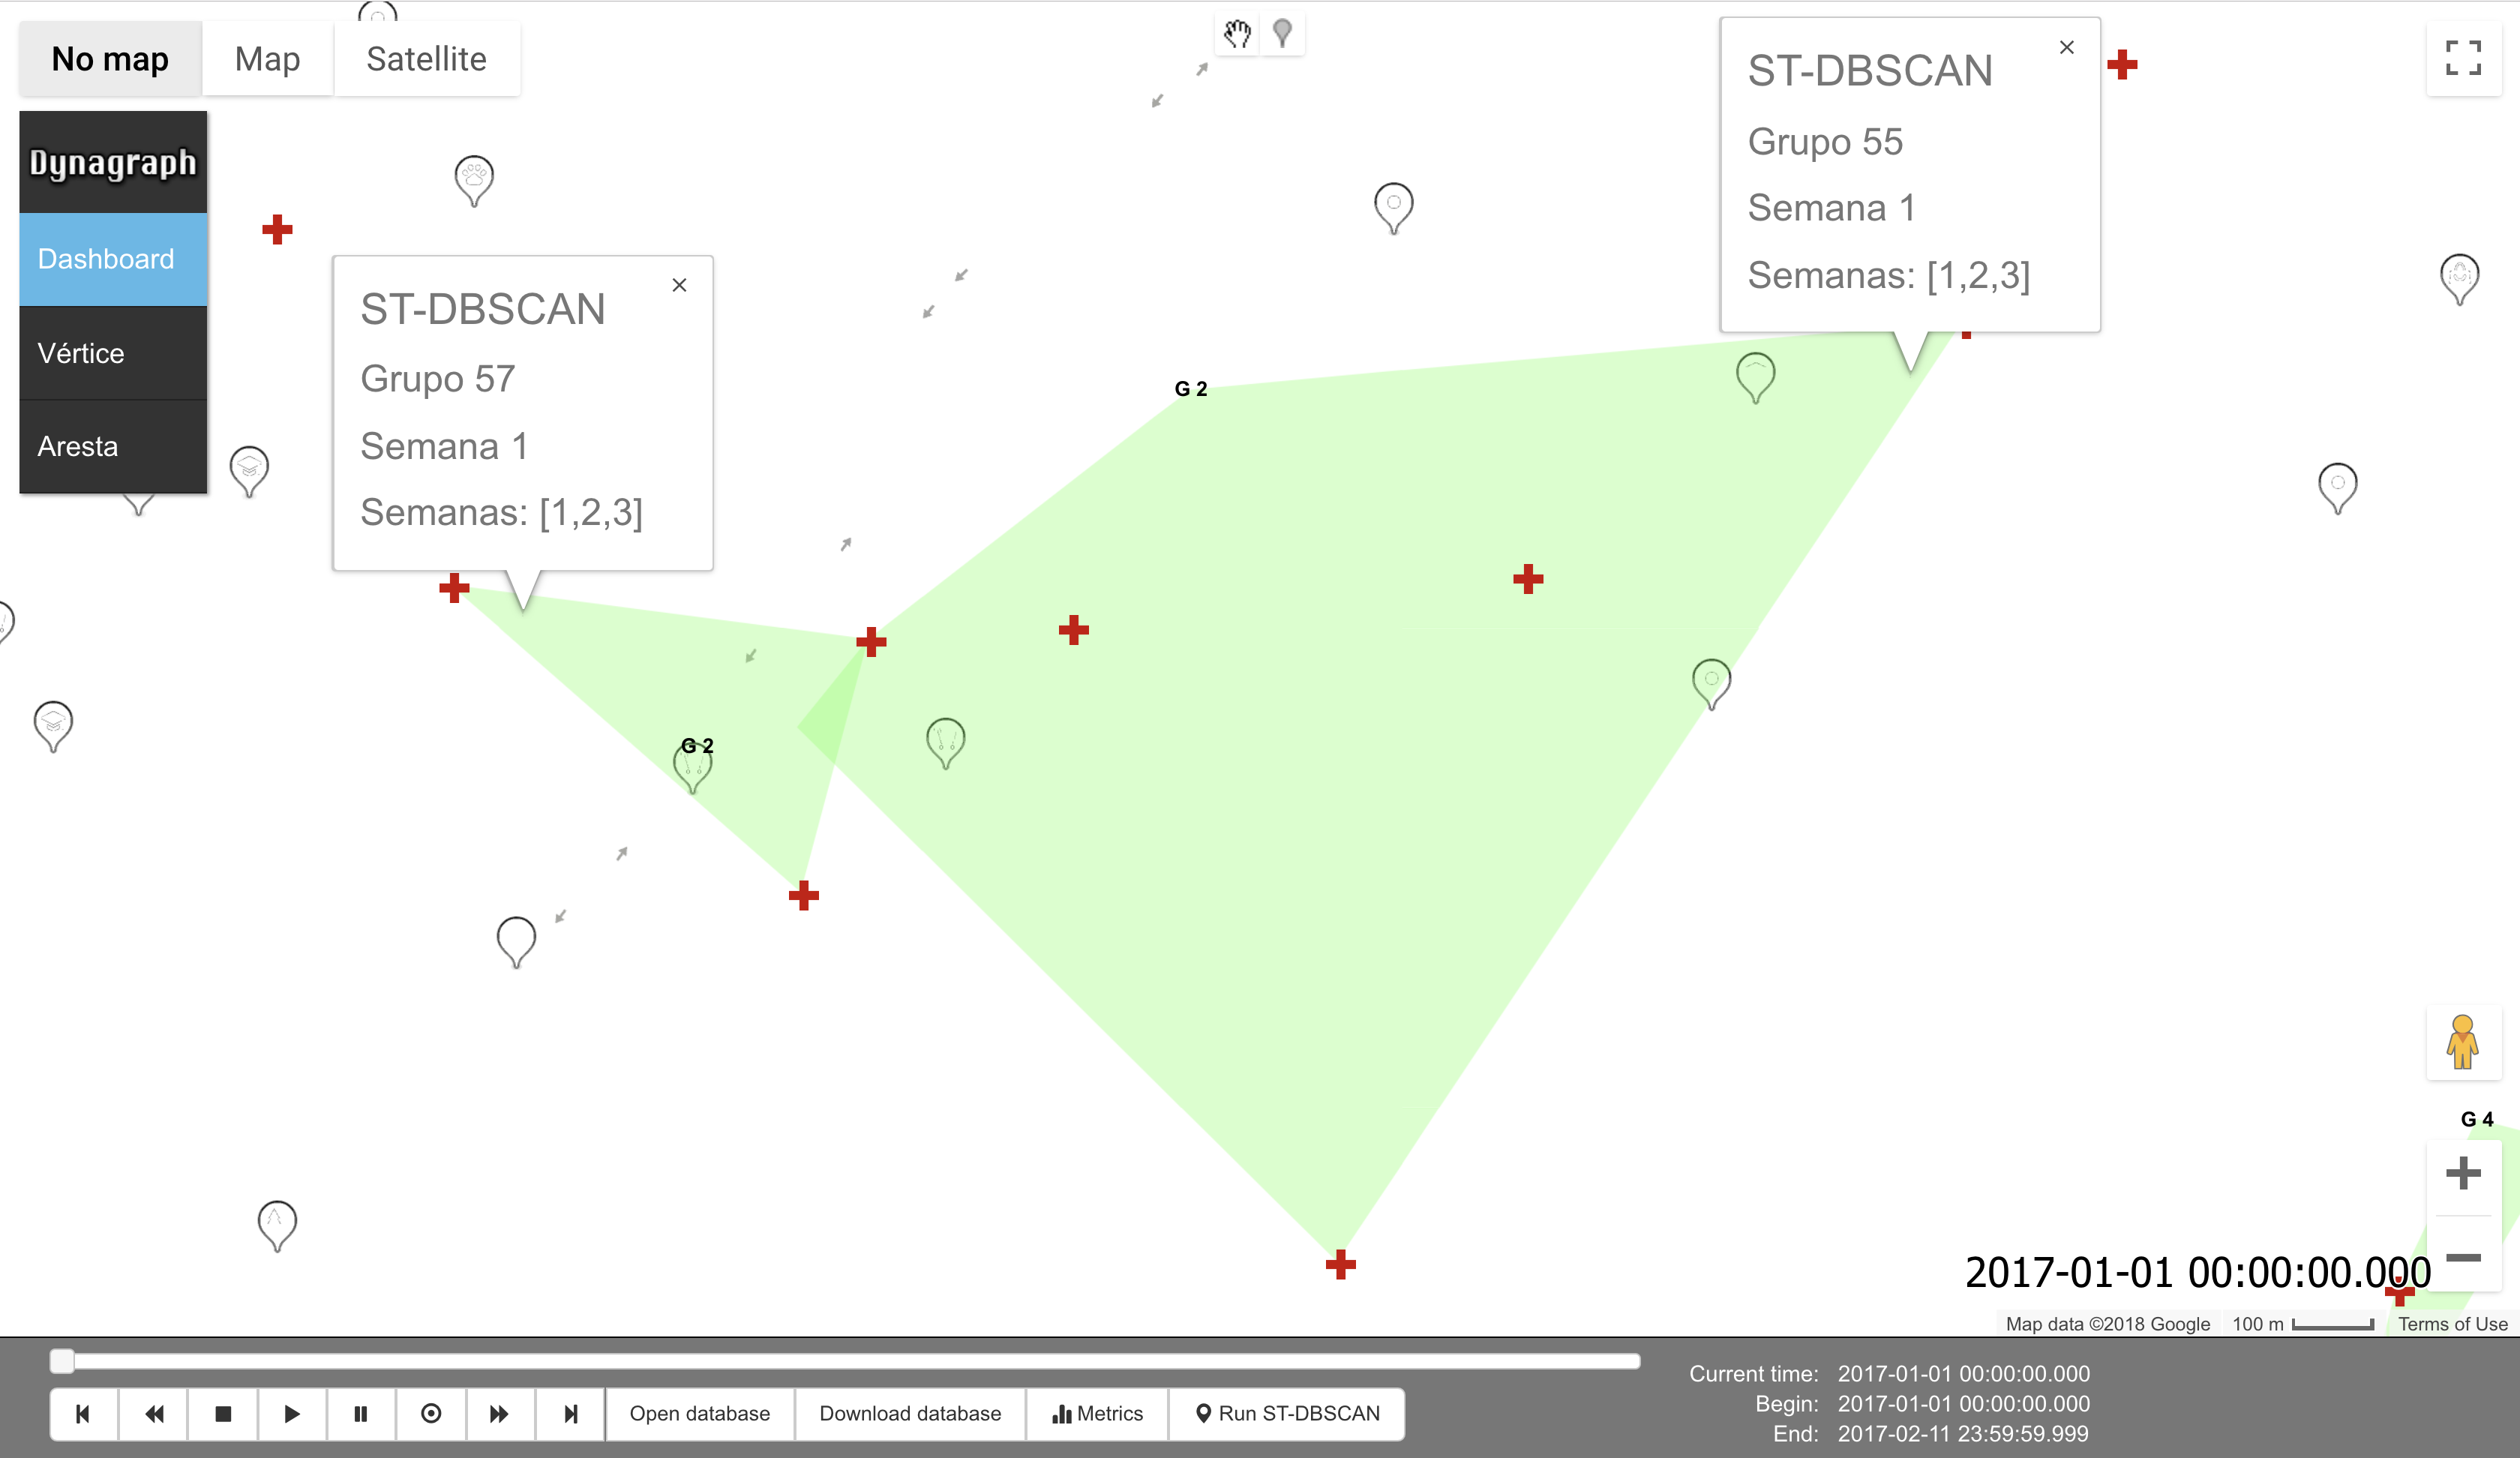
\includegraphics[width=15cm]{figuras/stdbscan/stdbscan1.png}
	}{
		\Fonte{Elaborado pelo autor}
	}
\end{figure}
\FloatBarrier

\begin{figure}[!ht]
	\centering	
	\Caption{\label{fig:stdbscan2} ST-DBSCAN: Semana 2}
	\UECEfig{}{
		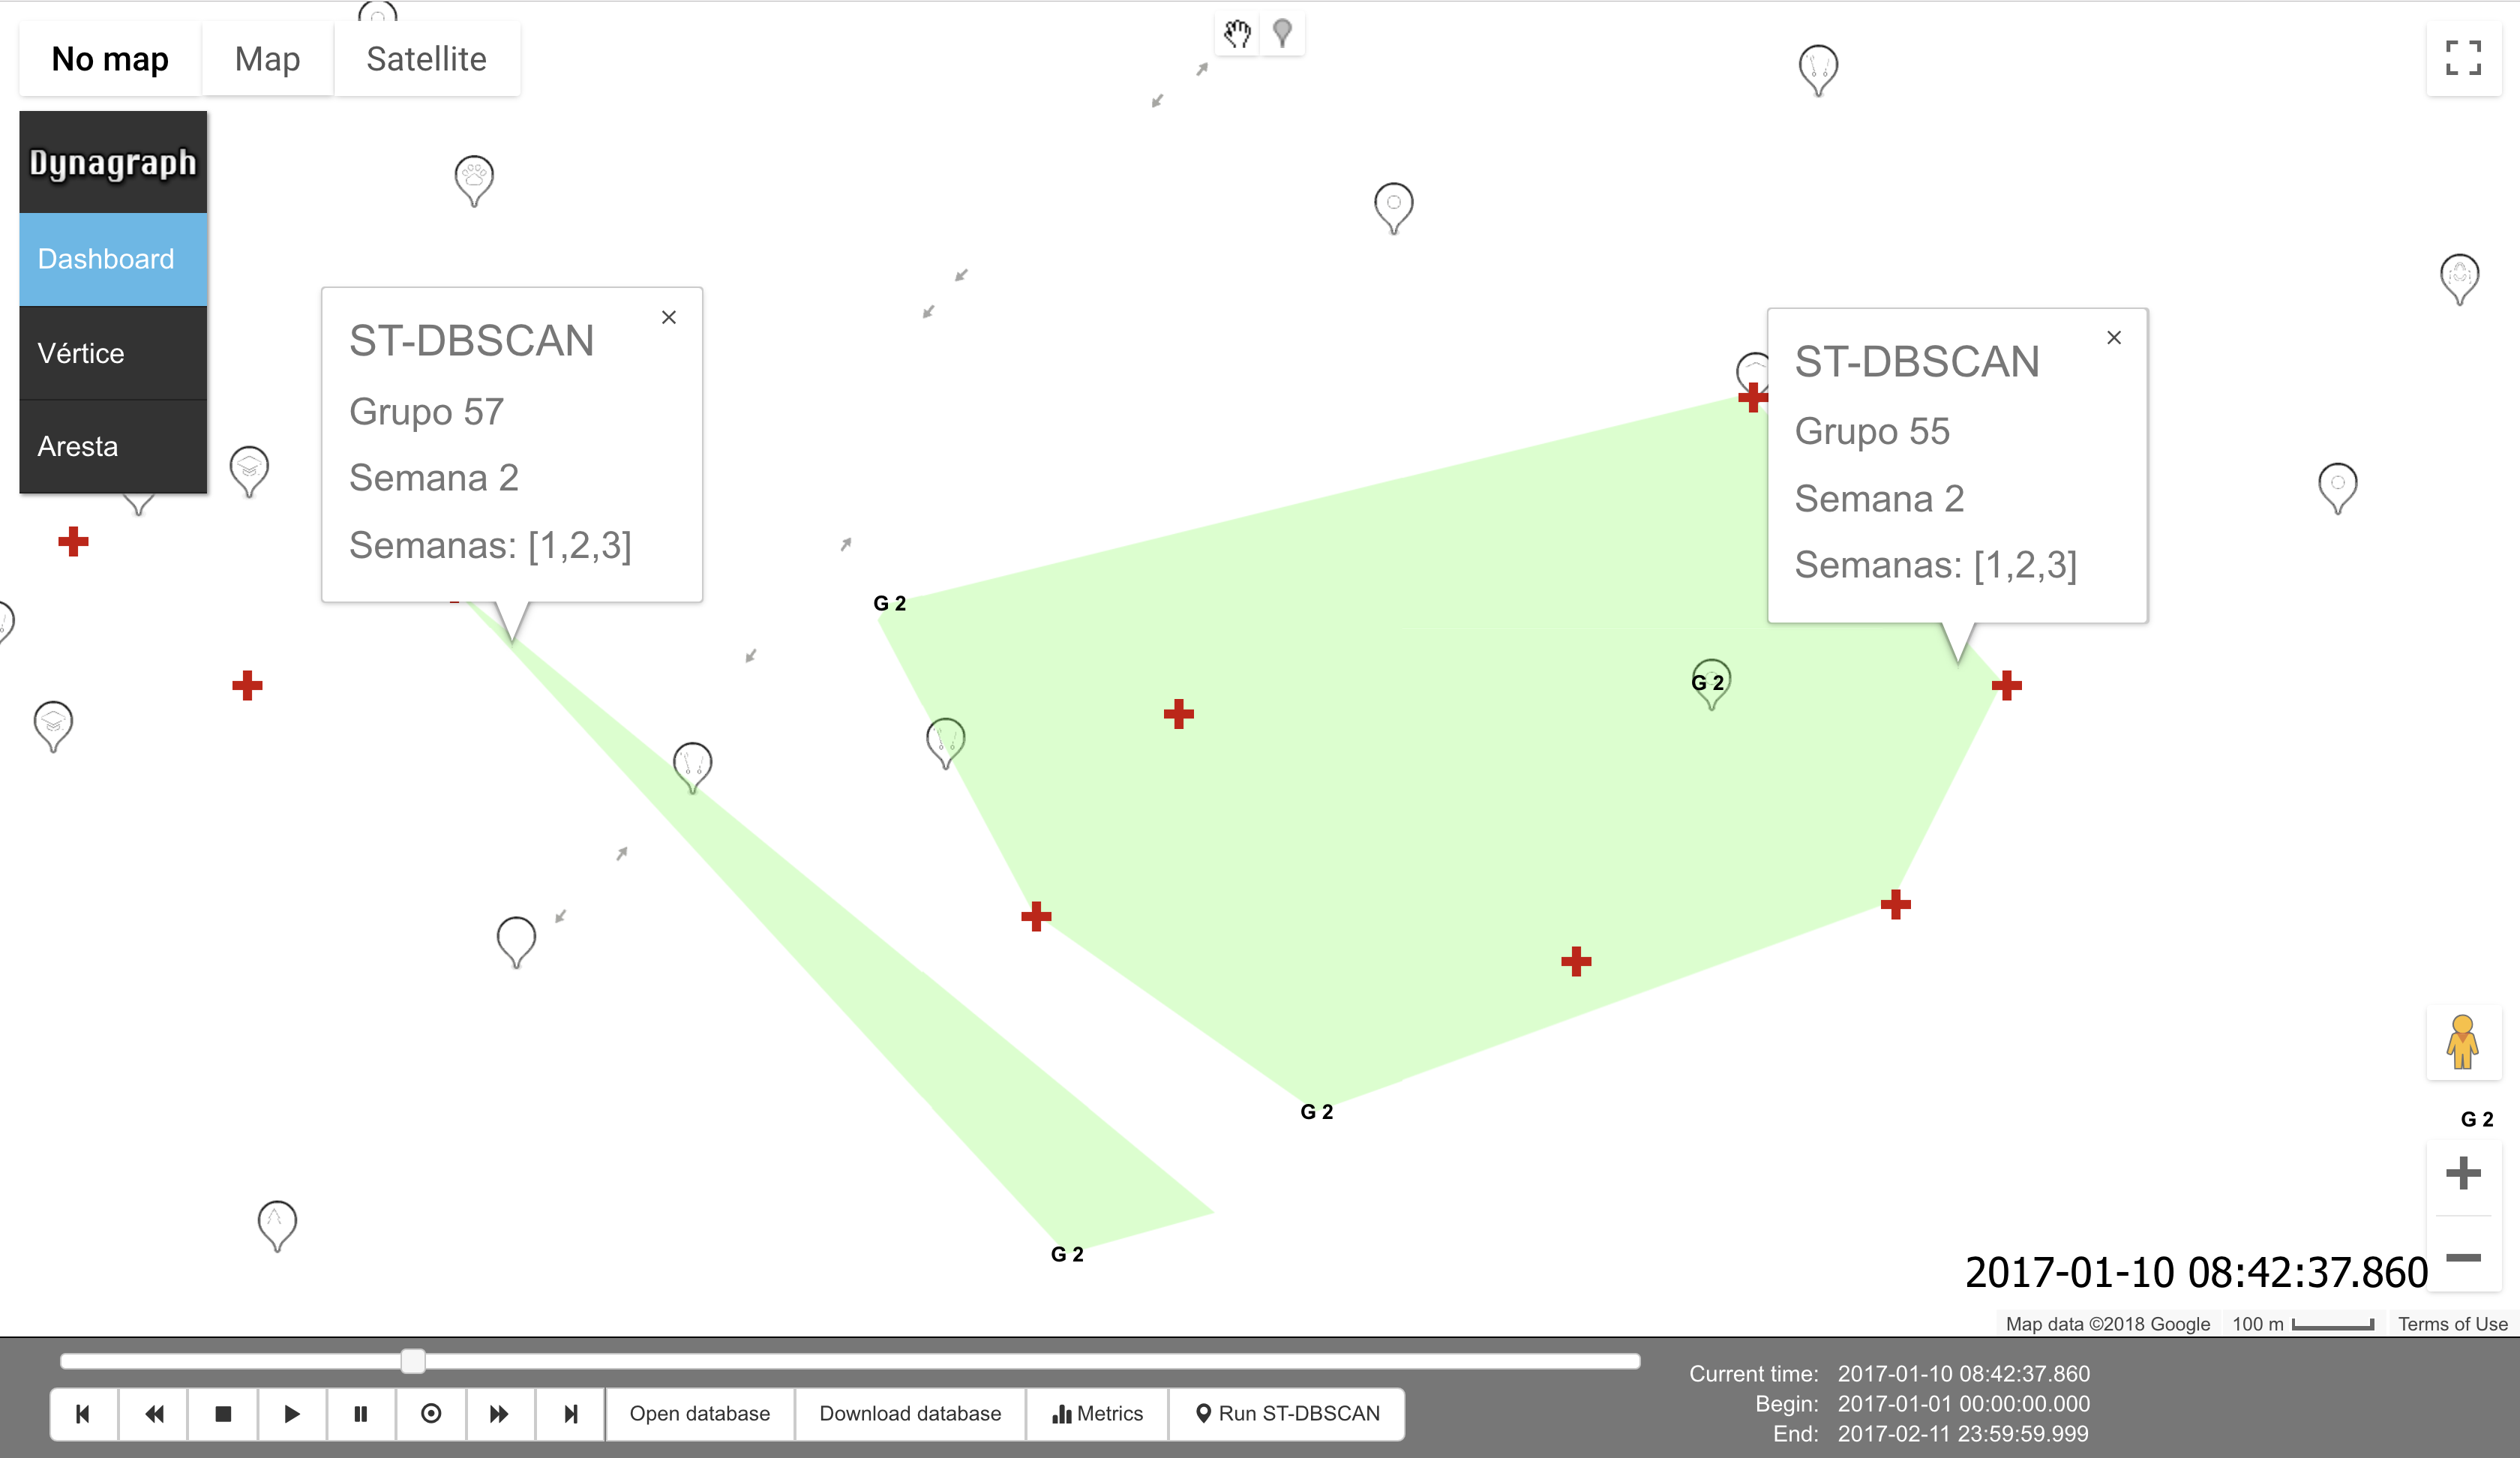
\includegraphics[width=15cm]{figuras/stdbscan/stdbscan2.png}
	}{
		\Fonte{Elaborado pelo autor}
	}
\end{figure}
\FloatBarrier

\begin{figure}[!ht]
	\centering	
	\Caption{\label{fig:stdbscan3} ST-DBSCAN: Semana 3}
	\UECEfig{}{
		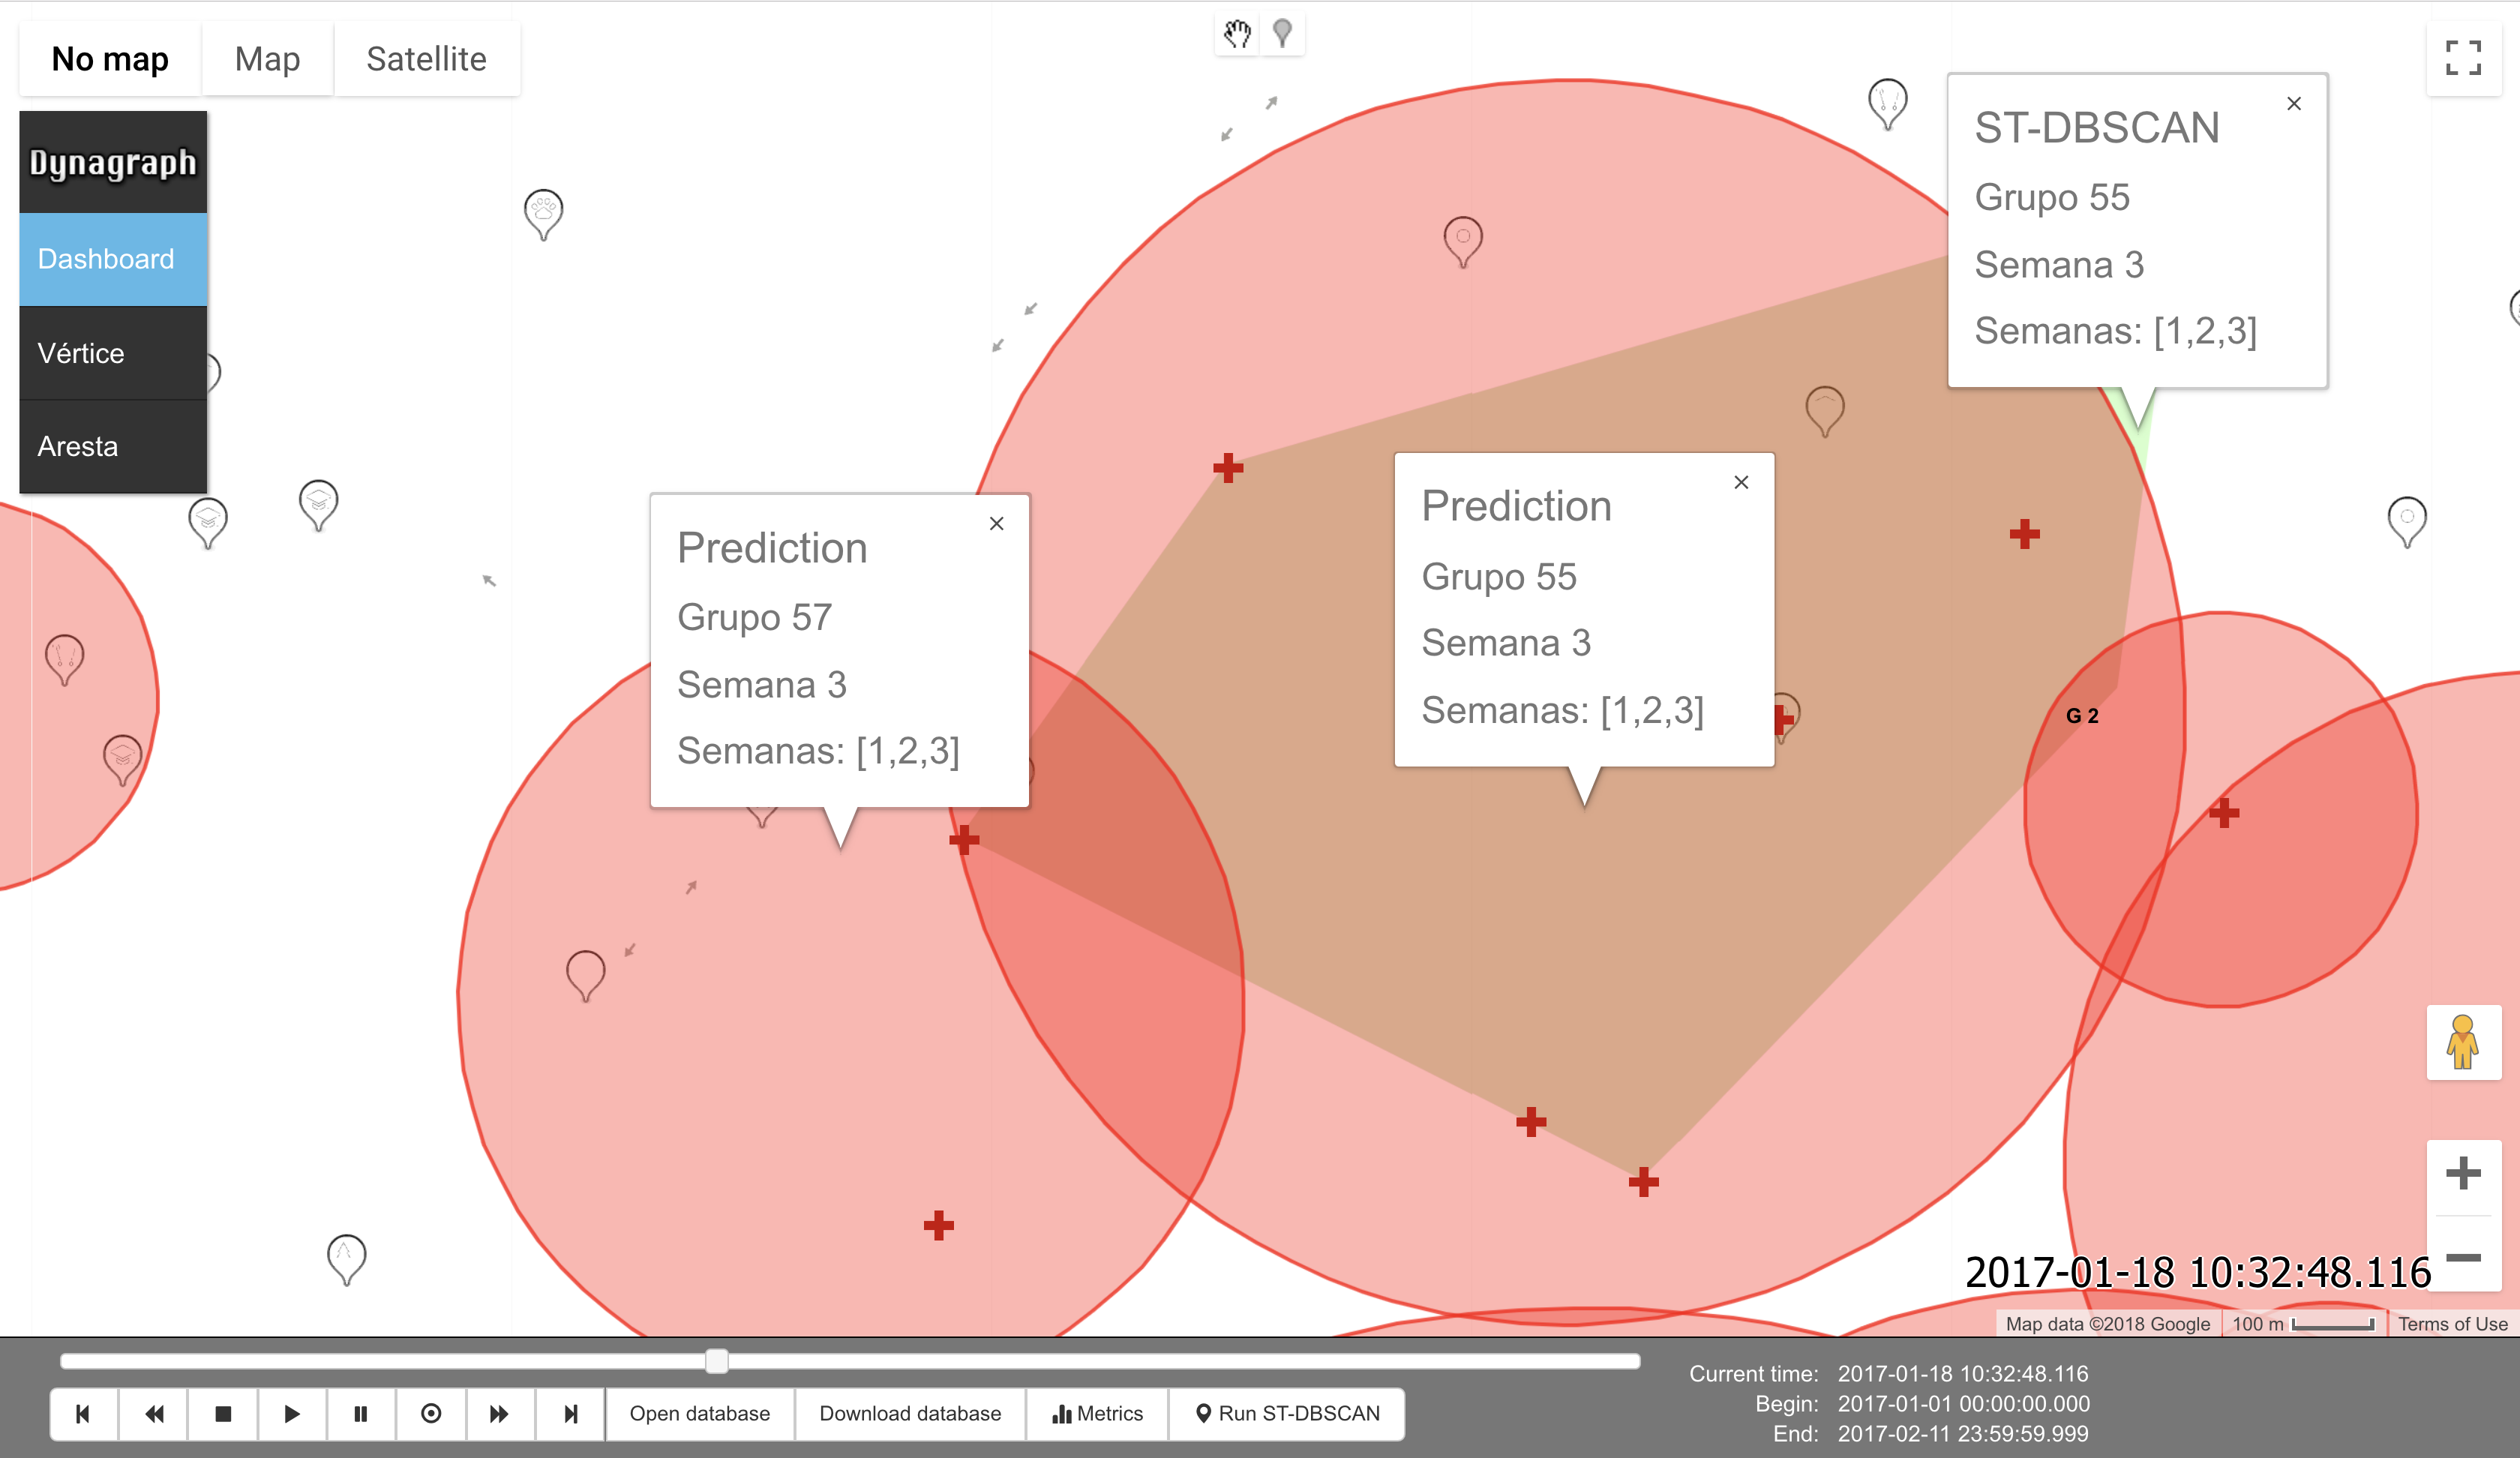
\includegraphics[width=15cm]{figuras/stdbscan/stdbscan3.png}
	}{
		\Fonte{Elaborado pelo autor}
	}
\end{figure}
\FloatBarrier